\section{Results}\label{sec:results}

All intervals are 95 percent intervals of the mean over seeds (Eq.~\ref{eq:ci}). The main experiment has \nSeeds{} seeds, the ablation \nSeedsAbl{}, the timing three.

\subsection{The front and the published points on the ten by ten task}\label{sec:res-front}

Figure~\ref{fig:front} shows the fronts of the \nSeeds{} seeds with the points of the five published methods, and Table~\ref{tab:main} gives the means. The front starts at the refined output of phase-fixed WGS, with an efficiency of \eStart{} and a uniformity of 1 to three decimals, and it ends at the efficient end with a largest efficiency of \eMaxFront{} (interval \eMaxFrontLo{} to \eMaxFrontHi) and a smallest uniformity of \uMinFront{} (interval \uMinFrontLo{} to \uMinFrontHi). Over the whole front the efficiency changes by \eMaxFrontDelta{} while the uniformity falls from 1 to about 0, so
the front is steep: a gain of a few percent in light is paid for with nearly all of the uniformity. Of the \nLambda{} points, \nParetoMean{} on average are non-dominated in the plane $(e,u)$ (from \nParetoMin{} to \nParetoMax{} across seeds), so every weight gives a distinct non-dominated point in almost every seed.

\begin{figure}[t]
\centering
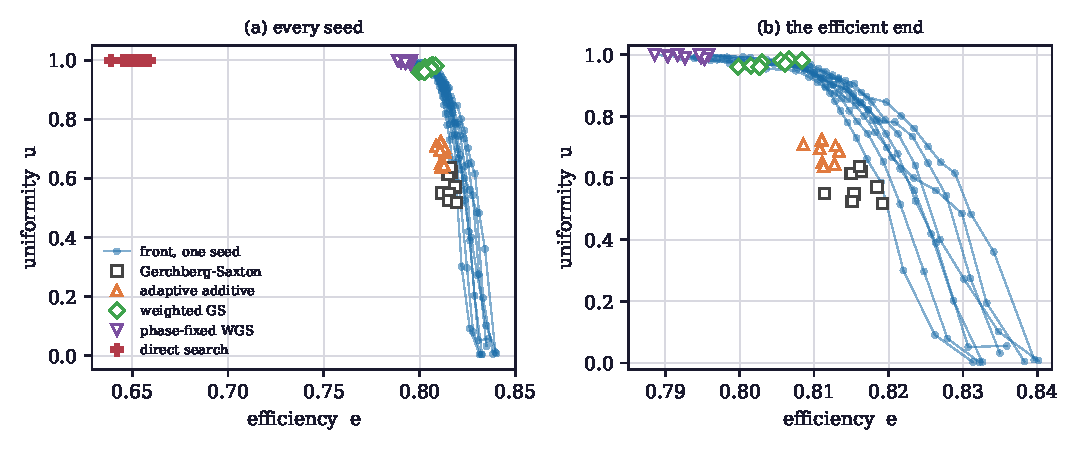
\includegraphics[width=\textwidth]{fig-front.pdf}
\caption{Fronts of the efficiency-uniformity trade-off on the ten by ten lattice for \nSeeds{} seeds (blue circles joined by lines) and the points of the five published methods on the same seeds (open and filled markers): (a) the whole plane, (b) enlarged near the efficient end. The front falls steeply from the uniform end, and the points of weighted GS, phase-fixed WGS and direct search sit near that end.}
\label{fig:front}
\end{figure}

\begin{table}[t]
\centering\small
\caption{Efficiency and uniformity (mean $\pm$ half-width of the 95 percent interval over \nSeeds{} seeds) of the points of the published methods and of the front on the ten by ten lattice, and the hypervolume with the reference $(0,0)$: for a single point it is $e\,u$, for the union of four points and for the front it is the area of Eq.~\ref{eq:hv}. The union is that of Gerchberg--Saxton, the adaptive additive iteration, weighted GS and direct search, without phase-fixed WGS.}
\label{tab:main}
\begin{tabular}{@{}lrrr@{}}
\toprule
Result & Efficiency & Uniformity & Hypervolume \\
\midrule
Gerchberg-Saxton & $0.816\pm0.002$ & $0.573\pm0.038$ & $0.468\pm0.031$ \\
Adaptive additive & $0.811\pm0.001$ & $0.682\pm0.027$ & $0.553\pm0.022$ \\
Weighted GS & $0.804\pm0.002$ & $0.972\pm0.008$ & $0.782\pm0.008$ \\
Phase-fixed WGS & $0.793\pm0.002$ & $0.995\pm0.004$ & $0.789\pm0.003$ \\
Direct search & $0.651\pm0.005$ & $0.999\pm0.000$ & $0.650\pm0.005$ \\
\midrule
Union of the four published points &  &  & $0.8071\pm0.0023$ \\
Front (knee point) & $0.793\pm0.002$ & $1.000\pm0.000$ &  \\
Front (whole) & 0.793 to 0.836 & 0.015 to 1 & $0.8223\pm0.0025$ \\
\bottomrule
\end{tabular}

\end{table}

The first hypothesis holds. The hypervolume of the front is \hvFront{} (interval \hvFrontCi) and that of the union of the four points is \hvPub{} (interval \hvPubCi), and the paired difference is \hvDiff{} with the interval \hvDiffLo{} to \hvDiffHi{}; it is positive in \hvGeCount{} of \nSeeds{} seeds, from \hvDiffMin{} in the weakest seed to \hvDiffMax{} in the strongest, which is a gain of \hvRatioPct{} percent of the union.
Adding phase-fixed WGS, the start of the front, to the union gives a hypervolume of \hvPubSeven{}, and the front still exceeds it by \hvDiffSeven{} (interval \hvDiffSevenLo{} to \hvDiffSevenHi) in \hvGeCountSeven{} of \nSeeds{} seeds. The union of the published points is not dominated by the front: the gain comes from the region of efficiency above the uniform end, where the front has points at intermediate uniformity that the published points leave empty, and not from a better uniform end. The second hypothesis holds: the front has \domGSMin{} to \domGSMax{} points that dominate the point of Gerchberg--Saxton (mean \domGSMean) and \domGAAMin{} to \domGAAMax{} that dominate the point of the adaptive additive iteration (mean \domGAAMean) in every seed, and
the number of seeds in which both are dominated is \domBothSeeds{} of \nSeeds{}. Direct search is dominated by one point of the front in \domDSSeeds{} of \nSeeds{} seeds, its efficiency of \ptDSE{} being the lowest of the five points.

The fourth hypothesis is not confirmed. The front has a dominating point for the point of weighted GS in only \domGSWSeeds{} of \nSeeds{} seeds (at most \domGSWMax{} points) and for the point of phase-fixed WGS in \domPFSeeds{} of \nSeeds{} (at most \domPFMax). The two points are the ones nearest the uniform end of the front: weighted GS has an efficiency of \ptGSWE{} and a uniformity of \ptGSWU{}, phase-fixed WGS \ptPFE{} and \ptPFU{}, while the front at the same efficiency has a lower uniformity. The reading is the risk that the research record named: the points of weighted GS are already near the best attainable corner on this task, and the front adds the efficient side of the trade-off and not a better uniform end.
The representative point of Eq.~\ref{eq:knee} is the uniform end in every seed, with an efficiency of \kneeE{} (interval \kneeELo{} to \kneeEHi) and a uniformity of \kneeU{}: because the efficiency rises by a few percent while the uniformity falls by a large factor, the product $eu$ is largest where the uniformity is one, so the knee rule returns the refined start and the information of the method is in the front and not in the knee.

\begin{figure}[t]
\centering
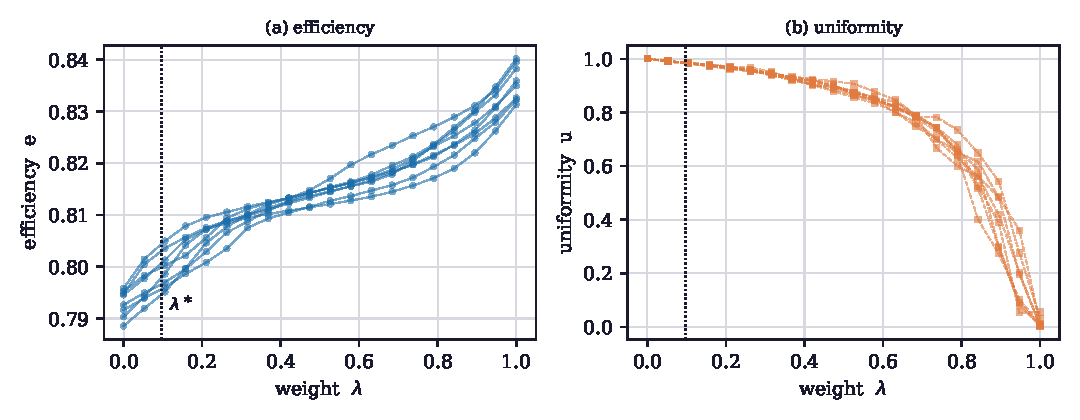
\includegraphics[width=\textwidth]{fig-lambda.pdf}
\caption{Efficiency (a) and uniformity (b) along the weight $\lambda$ for the \nSeeds{} seeds of the main experiment; the vertical dotted line is the mean value $\lambda^\ast$ of Eq.~\ref{eq:lamstar} computed from the largest efficiency of each front. The efficiency rises quickly up to about $\lambda=0.3$, slowly between 0.3 and 0.8 and quickly again near one; the uniformity falls slowly until $\lambda$ is near one, where it falls fast.}
\label{fig:lambda}
\end{figure}

Figure~\ref{fig:lambda} plots the two quantities against the weight. The efficiency increases monotonically with the weight in \monoESeeds{} of \nSeeds{} seeds, the error $E$ in \monoLossSeeds{} of \nSeeds{}, and the uniformity decreases monotonically in \monoUSeeds{} of \nSeeds{}, with at most \monoUViolMax{} step in which it rises in the remaining seed. This is the direction that Proposition~\ref{prop:mono}(a) predicts for global minimizers, here observed for the conjugate-gradient solutions. The weight at which the loss asks for the largest efficiency that is reached is
$\lambda^\ast=\lamSat{}$ (interval \lamSatLo{} to \lamSatHi). Beyond it the loss asks for more light than any hologram of the front delivers, and the front continues toward the efficient end: the efficiency still rises, up to a total gain of \eMaxFrontDelta{} over the start, and the uniformity falls from near one to near zero. The value of $\lambda^\ast$ is computed from the largest efficiency that each front reaches, so it restates that measurement as a weight and is not a prediction; the quantity that the proposition gives without a run is the upper bound $\lambda_1=\ablTargetLamMax{}$ (Section~\ref{sec:ablation}), which is well above the measured $\lambda^\ast$. The measured front shows that the supply keeps growing slowly after $\lambda^\ast$, at the price of the uniformity.

\subsection{Sensitivity to the reference point and one-parameter fronts of the published methods}\label{sec:res-rivals}

The hypervolume depends on the reference point. Table~\ref{tab:refs} repeats the comparison of the front and the published union with the reference $(0.5,0)$ and $(0.7,0)$, which discard the part of the plane below those efficiencies. The paired difference is \hvRefHalfDiff{} (interval \hvRefHalfLo{} to \hvRefHalfHi) and \hvRefSevenDiff{} (interval \hvRefSevenLo{} to \hvRefSevenHi) respectively, positive in \hvRefHalfGe{} and \hvRefSevenGe{} of \nSeeds{} seeds, so the ordering does not depend on the reference among the three tested. The size of the difference
is about the same in absolute terms for the three references, while the hypervolumes themselves shrink, so in relative terms the front's advantage grows as the reference moves toward the efficiencies at which the methods operate. The hypervolume with the reference $(0,0)$ is dominated by the high-uniformity region, where a point already covers most of the area, which is the weakness of the criterion that the acceptance test of the method inherits.

\begin{table}[t]
\centering\small
\caption{Hypervolume of the front and of the union of the four published points for three reference points, with the paired difference (mean $\pm$ half-width of the 95 percent interval over \nSeeds{} seeds). The ordering of the front and the union is the same for the three references.}
\label{tab:refs}
\begin{tabular}{@{}lrrr@{}}
\toprule
Reference of the hypervolume & Front & Published union & Difference, 95\% interval \\
\midrule
$(0,0)$ & $0.8223\pm0.0025$ & $0.8071\pm0.0023$ & $0.0152\pm0.0027$ \\
$(0.5,0)$ & $0.3223\pm0.0025$ & $0.3074\pm0.0023$ & $0.0149\pm0.0027$ \\
$(0.7,0)$ & $0.1223\pm0.0025$ & $0.1088\pm0.0020$ & $0.0135\pm0.0025$ \\
\bottomrule
\end{tabular}

\end{table}

A single point of a published method is a weak comparator, because each method has a knob that moves it. The one-parameter fronts of Section~\ref{sec:compared} give the published methods their best chance: the iterates of weighted GS and of phase-fixed WGS, and the sweep of the exponent of the adaptive additive iteration. Table~\ref{tab:rivals} gives their hypervolume. The front exceeds the weighted GS path by \rivGswDiff{} (interval \rivGswLo{} to \rivGswHi), the phase-fixed path by \rivPfDiff{} (\rivPfLo{} to \rivPfHi) and the adaptive additive sweep by \rivGaaDiff{} (\rivGaaLo{} to \rivGaaHi), in \rivGswGe{}, \rivPfGe{} and \rivGaaGe{} of \nSeeds{} seeds, and it exceeds the union of all of them and of the five points by \rivUnionDiff{} (interval \rivUnionLo{} to \rivUnionHi{}) in \rivUnionGe{} of \nSeeds{} seeds.
The fifth hypothesis therefore holds on the hypervolume. It does not mean that the front is better than the published methods point by point. Figure~\ref{fig:rivals} shows why. The iterates of weighted GS approach a point that lies on the uniform side of the front with a higher efficiency than the front has at the same uniformity: in seed 1, weighted GS after 100 iterations reaches an efficiency of \seedOneGswE{} at a uniformity of \seedOneGswU{}, while the front point of nearest efficiency (\seedOneNearE) has a uniformity of \seedOneNearU{}. Of the \nLambda{} points of the front, \frontDomMin{} to \frontDomMax{} (mean \frontDomMean) are dominated by at least one point of the published methods and their one-parameter fronts, and adding the published points to the front raises its hypervolume by only \hvGainPub{} on average (at most \hvGainPubMax). Of the 211 points of the three one-parameter fronts, \rivUndom{} on average per seed (at most \rivUndomMax) have no front point of equal or higher efficiency and uniformity, which says that the front does not cover the published iterates.

\begin{table}[t]
\centering\small
\caption{Hypervolume of the one-parameter fronts that the published methods give on the same seeds, the paired difference of the front from each (mean $\pm$ half-width of the 95 percent interval), and the number of seeds in which the front is at least as large. The last row is the union of the three fronts and of the five points.}
\label{tab:rivals}
\begin{tabular}{@{}lrrr@{}}
\toprule
One-parameter front of a published method & Hypervolume & Front minus it & Seeds front $\ge$ \\
\midrule
Weighted GS, iterates 1 to 100 & $0.8054\pm0.0020$ & $0.0169\pm0.0037$ & 8 of 8 \\
Phase-fixed WGS, iterates 1 to 100 & $0.7899\pm0.0034$ & $0.0324\pm0.0050$ & 8 of 8 \\
Adaptive additive, exponent 0 to 1 & $0.5880\pm0.0172$ & $0.2343\pm0.0158$ & 8 of 8 \\
Union of all of them and the five points & $0.8131\pm0.0012$ & $0.0092\pm0.0016$ & 8 of 8 \\
\bottomrule
\end{tabular}

\end{table}

\begin{figure}[t]
\centering
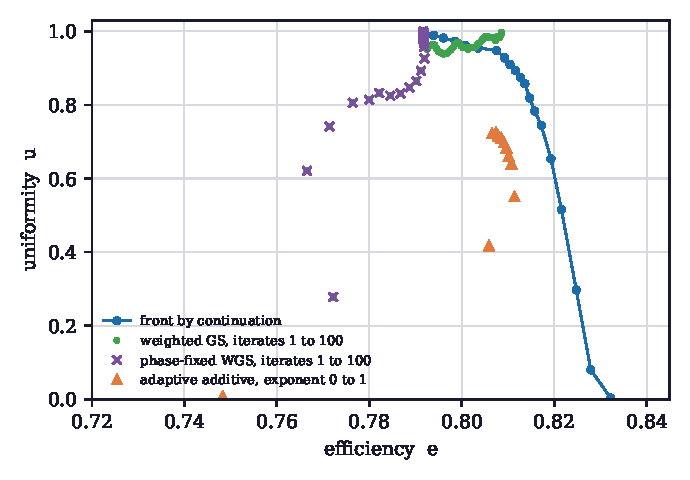
\includegraphics[width=0.78\textwidth]{fig-rivals.pdf}
\caption{The front of seed 1 (blue circles joined by a line) against the iterates 1 to 100 of weighted GS (green dots) and of phase-fixed WGS (purple crosses), and the adaptive additive iteration at 30 iterations with the exponent from 0 to 1 (orange triangles), on the ten by ten lattice. The last iterates of weighted GS lie above and to the right of the first points of the front.}
\label{fig:rivals}
\end{figure}

The dominance of part of the front by published iterates depends on the iteration budget and on the start, and not only on the loss: with 30 conjugate-gradient iterations per weight instead of 15 the mean number of dominated points falls from \ablDefaultDom{} to \ablCgThirtyDom{}, and when the front starts from the hologram of weighted GS after 100 iterations it falls to \ablStartGswHDom{} (Section~\ref{sec:ablation}), on the five seeds of the ablation. A direct comparison on the loss itself separates two explanations. The hologram of weighted GS after 100 iterations has a normalized error $E$ of \diagGswHundredE{} and a normalized light $S$ of \diagGswHundredS{} on the target of the seed, and for \diagGswHundredSeeds{} of \nSeeds{} seeds there is at least one weight at which its loss $L_\lambda$ is lower than that of the front
point (\diagGswHundredMin{} to \diagGswHundredMax{} weights, mean \diagGswHundredMean). The conjugate-gradient minimizer of the loss therefore stops, at those weights, in a point that is worse on the loss itself than a hologram that the fixed-point iteration of weighted GS reaches; the first part of the front inherits the basin of its start. The same comparison for phase-fixed WGS after 100 iterations gives \diagPfHundredSeeds{} of \nSeeds{} seeds with at least one weight (mean \diagPfHundredMean{} weights).

\subsection{What the weight does: the shifted target and the bounds}\label{sec:res-theory}

Figure~\ref{fig:shift}(a) draws the total light that the shifted target of Proposition~\ref{prop:shift} asks for, as a multiple of the efficiency of the start, and panel (b) plots the efficiency that the hologram reaches against it for the \nSeeds{} seeds. The two do not agree: the requested total grows with the weight without bound, while the efficiency reached stays within a few percent of the start. The measured efficiency at the largest weight is \eMaxFront{}, \eMaxRatio{} times the efficiency of the start, and the shifted target passes that value at the weight
$\lambda^\ast=\lamSat{}$. The gap between what is asked and what is delivered is the price of keeping the traps equal: the loss raises the target of every trap by the same amount, and a phase-only hologram on this task cannot follow it with a gain of more than \eMaxRatioPct{} percent in light.

\begin{figure}[t]
\centering
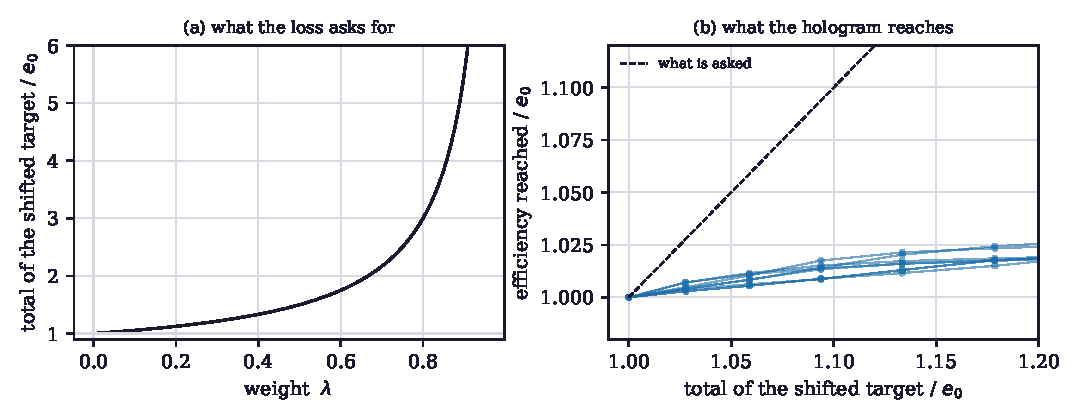
\includegraphics[width=\textwidth]{fig-shift.pdf}
\caption{(a) Total light of the shifted target of Proposition~\ref{prop:shift} as a multiple of the efficiency of the start, against the weight $\lambda$ (equal weights). (b) Efficiency reached by the hologram at each weight, as a multiple of the efficiency of the start, against the total that the target asks for, for the \nSeeds{} seeds; the dashed line is the case in which the hologram delivers what is asked.}
\label{fig:shift}
\end{figure}

The bounds of Proposition~\ref{prop:bound} hold on every front point of every seed. The smallest slack of the first bound, the bound minus the measured relative standard deviation in percent, is \sigmaSlackMin{}, which is positive and close to zero because the bound is an equality where the efficiency equals that of the start, as at the first point of each front. The smallest slack of the second bound is \uSlackMin{}; the bound is informative, that is, above zero, on \uBoundInf{} of the \uBoundPts{} front points of the main experiment, the ones with small error. Figure~\ref{fig:bound} plots the first bound.
A numerical check of the identity of Proposition~\ref{prop:shift} on random phases of a small array gives a largest absolute residual of \identResid{} over \identTrials{} trials and five weights, at the level of the rounding of the arithmetic.

\begin{figure}[t]
\centering
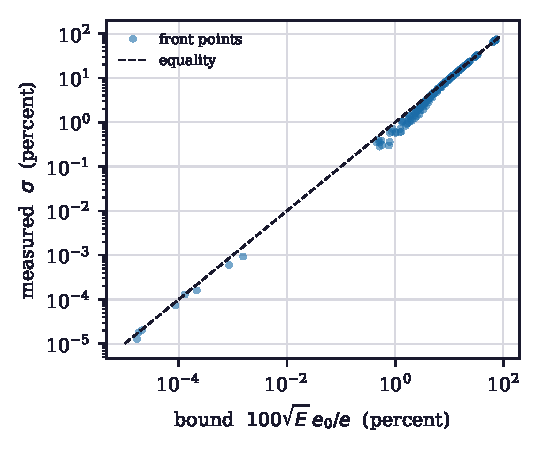
\includegraphics[width=0.62\textwidth]{fig-bound.pdf}
\caption{Relative standard deviation $\sigma$ of every front point of the main experiment (blue dots) against the bound of Proposition~\ref{prop:bound}, $100\sqrt E\,e_0/e$ (both in percent, logarithmic axes), and the line of equality (dashed). Every point is on or below the line; the points near the line are those whose efficiency is close to that of the start.}
\label{fig:bound}
\end{figure}

\subsection{Cost of the front}\label{sec:res-cost}

The third hypothesis concerns the time. Alone on the machine and with the module's own entry, the front takes \timeAloneMin{} to \timeAloneMax{} seconds for the three timed seeds (mean \timeAlone), so it is under the 60 seconds of the acceptance criterion in \timeAloneUnder{} of \timeAloneN{} seeds, with a margin that is thin on this machine and that the load of the machine changes. The record of the engine reports 16.6 seconds for the same task, a factor of about three below these times; this paper does not explain the factor: the timing here ran on a machine shared with other jobs (Section~\ref{sec:limits}), and the machine and the load of that record are not available to this paper, so the two times are not comparable and only the criterion of 60 seconds is read from the present ones. Over the \timeN{} runs of the ablation, the seconds in one thread are described by a line of $\timeSlope\,$ms
per conjugate-gradient iteration of one weight plus a constant of \timeIntercept{} seconds (coefficient of determination \timeRTwo), shown in Figure~\ref{fig:cost}. The constant is the part of the cost that does not scale with the weights and steps, mainly the start of 30 iterations of phase-fixed WGS, and the slope is the cost of one conjugate-gradient iteration, one to a few evaluations of the loss and its gradient; the linear model of Eq.~\ref{eq:cost} describes the measured time well. A direct search sweep on the same task takes \dsSec{} seconds in one thread, about as long as the whole front, and
the front returns \nParetoMean{} points where a sweep returns one.

\begin{figure}[t]
\centering
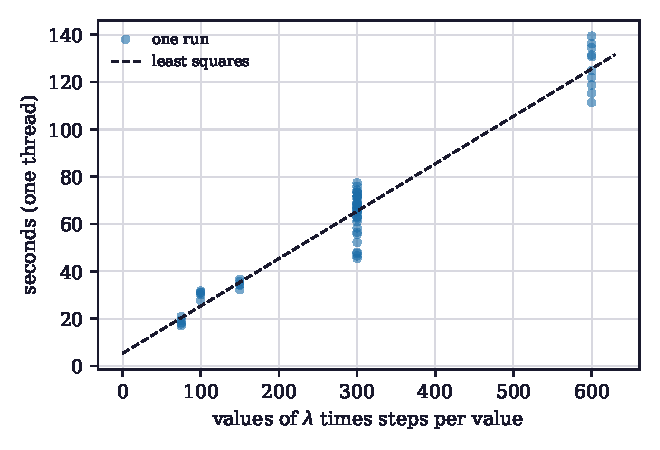
\includegraphics[width=0.62\textwidth]{fig-cost.pdf}
\caption{Seconds of one front in one thread against the number of weights times the conjugate-gradient iterations per weight, for the runs of the ablation (blue dots) and the least-squares line (dashed). The runs differ in the number of weights and the steps per weight; the line fits them with the coefficient of determination stated in the text.}
\label{fig:cost}
\end{figure}

\subsection{Other geometries: the benchmark and the bake}\label{sec:res-bench}

The benchmark of the studio stores a front for \benchNThirty{} of its geometries, obtained from the first seed with the converged budget, and the published points of the same geometry from the medians of the cells at 30 and 100 iterations on the ideal device. Table~\ref{tab:bench} gives the hypervolume of the stored front, that of the union of the four published points and the difference, and Figure~\ref{fig:bench} plots the difference. At 30 iterations the front meets the union on \benchPassThirty{} of \benchNThirty{}
geometries, with margins from \benchWorstThirty{} to \benchBestThirty{}. At 100 iterations it meets it on \benchPassHundred{} of \benchNHundred{}, with margins from \benchWorstHundred{} to \benchBestHundred{}, so the stored front lies below the union by at most \benchWorstAbsHundred{}. The eighth hypothesis is therefore refuted on the stored data at both budgets: the worst margin is \benchWorstThirty{} at 30 iterations and \benchWorstHundred{} at 100. Two facts qualify the result. The stored fronts are truncated: each ends at a weight below one (the largest stored weight is in Table~\ref{tab:bench}), which is consistent with the wall-clock limit of the converged
row of the benchmark, so the front misses the efficient tail that contributes to the hypervolume. And the medians of the published points are those of the cells of the benchmark, whose seeds depend on the wall-clock bound; the count of geometries at 100 iterations moved between runs of the benchmark of the same release, from 3 to 4 and to 0 in the record of the engine, and the file that is read here gives \benchPassHundred{}.

\begin{table}[t]
\centering\small
\caption{Hypervolume of the stored front of each benchmark geometry that has one, that of the union of the medians of the four published points (Gerchberg--Saxton, adaptive additive, weighted GS, direct search), and their difference, at 30 and at 100 iterations on the ideal device; the number of stored points and the largest stored weight are listed. Source: the committed benchmark file.}
\label{tab:bench}
\footnotesize\setlength{\tabcolsep}{3pt}
\begin{tabular}{@{}llrrrrr@{}}
\toprule
Geometry & Iter. & Points & Largest $\lambda$ & Front & Union & Difference \\
\midrule
G1 lattice 10 x 10 & 30 & 3 & 0.105 & 0.8352 & 0.8270 & +0.0082 \\
G2 ring, 36 traps & 30 & 7 & 0.368 & 0.7082 & 0.6966 & +0.0116 \\
G3 random, 100 traps & 30 & 6 & 0.263 & 0.7144 & 0.7041 & +0.0103 \\
G4 quasi-periodic, 119 & 30 & 5 & 0.211 & 0.7708 & 0.7643 & +0.0065 \\
G5 3D lattice 5 x 5 x 3 & 30 & 5 & 0.211 & 0.9012 & 0.8876 & +0.0136 \\
G6 large, 1024 and 819 & 30 & 1 & 0.000 & 0.7910 & 0.7916 & -0.0006 \\
G1 lattice 10 x 10 & 100 & 3 & 0.105 & 0.8352 & 0.8395 & -0.0043 \\
G2 ring, 36 traps & 100 & 7 & 0.368 & 0.7082 & 0.7017 & +0.0065 \\
G3 random, 100 traps & 100 & 6 & 0.263 & 0.7144 & 0.7106 & +0.0039 \\
G4 quasi-periodic, 119 & 100 & 5 & 0.211 & 0.7708 & 0.7718 & -0.0010 \\
G5 3D lattice 5 x 5 x 3 & 100 & 5 & 0.211 & 0.9012 & 0.8985 & +0.0026 \\
G6 large, 1024 and 819 & 100 & 1 & 0.000 & 0.7910 & 0.8037 & -0.0127 \\
\bottomrule
\end{tabular}

\end{table}

\begin{figure}[t]
\centering
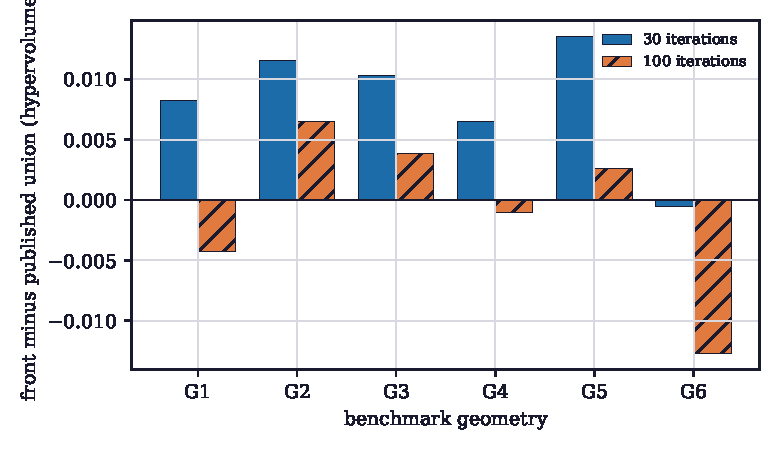
\includegraphics[width=0.8\textwidth]{fig-bench.pdf}
\caption{Hypervolume of the stored front minus that of the union of the four published points for each benchmark geometry, at 30 iterations (solid bars) and at 100 iterations (hatched bars). Bars above zero mean the front covers more area than the points; at 100 iterations \benchPassHundred{} of the \benchNHundred{} bars are at or above zero.}
\label{fig:bench}
\end{figure}

Table~\ref{tab:bake} lists the knee of the front that the studio's bake stores for the cases that run the method, as the mean and the interval over \bakeSeeds{} seeds. The knee is the refined start in the four cases (an efficiency near that of phase-fixed WGS on the cases of one plane and a uniformity near one), and the relative standard deviation is below one percent in every case listed, so the bake shows the uniform end of the front and not its trade-off.

\begin{table}[t]
\centering\small
\caption{Knee of the front stored by the studio's bake for the cases that run the method: efficiency, uniformity and relative standard deviation (mean $\pm$ half-width of the 95 percent interval over \bakeSeeds{} seeds; the intervals are wide with three seeds). Source: the committed file of measured ranges.}
\label{tab:bake}
\begin{tabular}{@{}lrrr@{}}
\toprule
Case & Efficiency & Uniformity & Relative std. dev. (percent) \\
\midrule
C01 & $0.801\pm0.066$ & $1.000\pm0.002$ & $0.03\pm0.13$ \\
C02 & $0.803\pm0.017$ & $0.989\pm0.030$ & $0.53\pm1.41$ \\
C05 & $0.895\pm0.015$ & $0.985\pm0.009$ & $0.66\pm0.39$ \\
C07 & $0.799\pm0.011$ & $0.990\pm0.017$ & $0.54\pm0.98$ \\
\bottomrule
\end{tabular}

\end{table}

\subsection{Outcome of each hypothesis}\label{sec:res-outcome}

The first, second, third, fifth, sixth and seventh hypotheses hold on the task of the acceptance test. The first holds with a paired difference of \hvDiff{} in \hvGeCount{} of \nSeeds{} seeds, the second in every seed, the third with a thin margin on the machine used, the fifth with the front above the union of the one-parameter fronts, the sixth with monotone efficiency and error in every seed and a uniformity that rises once in one seed, and the seventh with the cold start lower by the amount of Table~\ref{tab:ablation}.
The fourth is not confirmed: the weighted GS and phase-fixed points are dominated in \domGSWSeeds{} and \domPFSeeds{} of \nSeeds{} seeds. The eighth is refuted on the benchmark at both budgets. The scope of the result is therefore the following. On the ten by ten task the front adds the efficient side of the trade-off to the points of the published methods and exceeds the area that those points and their one-parameter fronts cover, and it does not improve on the weighted GS iterates at the uniform end, where
\frontDomMin{} to \frontDomMax{} of its points are dominated.
